\documentclass[12pt]{article}

\usepackage{lastpage} % Required to determine the last page for the footer
\usepackage{extramarks} % Required for headers and footers
\usepackage{graphicx} % Required to insert images
\usepackage{listings} % Required for insertion of code
\usepackage{courier} % Required for the courier font
\usepackage{color}

% Margins
\topmargin=-0.45in
\evensidemargin=0in
\oddsidemargin=0in
\textwidth=6.5in
\textheight=9.0in
\headsep=0.25in

\linespread{1.1} % Line spacing

\vspace{4em}

\newcommand{\Title}{Software Architecture Specification Document} % Assignment title
\begin{document}

	\begin{center}%
		\LARGE \bf \Title \\[2em]
		\Large {Project:}\\
		Financial markets simulation with multiple competing algorithmic trading entities.\\[0.7em]
		\Large {Client:}
		Cortical Systems\\[2em]
		\LARGE {\bf Group:}\\
			\begin{figure}[ht!]
				\centering
				
\includegraphics[scale=0.4]{Logo8.png}
			\end{figure}
			
		\Large {\bf Members:}\\[0.3em]
		\large
		Daniel Makgonta 12147100\\
		Moeletji Semenya 12349136\\
		Madimetja Shika 12127877\\[3em]
	
	\small Publication Date: 21 May 2014\\[0.5em]
	\small Version: 0.0 		    
	\end{center}%
	
	\newpage		
	\large 
 	{\bf Change Log}\\[1em]
	\begin{tabular}{llll}
		Date & Name & Reason & Version \\
		13/05/2014 & Moeletji & Creation & 0.0 \\
		16/05/2014 & Moeletji & Adding functional requirements & 0.0 \\
		19/05/2014 & Daniel & Adding architectural requrements & 0.0 \\
		21/05/2014 & Madimetja & Editing & 0.0
	\end{tabular}
	

	
	\newpage
	\tableofcontents
				  
	\newpage
	\section{Architectural requirements}	    
			    \subsection{Architectural scope}	
			    	   \begin{itemize}
			    	   		\item The Java programming language will be used for main process execution and C/C++ languages will be used as dll references within the Java classes to 
			    	   		\item JDBC and MySQL are the database that will be used for the persistent infrastructure. 
			    	   		\item All reporting functions will be use JReport(Java Report).
			    	   		\item Graphs will be displayed using Java libraries Graphics2D, AWT and Swings. 
			    	   \end{itemize}
			    
			    \subsection{Quality requirements}	
			    	\subsubsection{Security}
			    	\begin{itemize}
			    		\item Only system administrators may view the statistical analysis of the system. 
			    		\item Only system administrators may tweak trading algorithms or matching engine to follow current trends within the stock market.
				   		\item Only registered users may be able to buy/sell shares on the system.
			       		\item The system allows anonymity in terms of no buyer or seller can view what another buyer or seller’s activities.
			       		\item Matching engine is only allowed to be accessed directly by system administrators. The matching engine is abstracted to the buyers and sellers of the system.  
			       		\item System administrators are not allowed to participate in the trading simulation.
			    	\end{itemize}	
			    		
			    	\subsubsection{Auditability}
			    	\begin{itemize}
				    	\item One should be able to query any entity within the system, this includes the user who made the change, the data that was changed, the new and old values of the data, as well as when the data was changed.
			    	\end{itemize}
			    	
			    	\subsubsection{Testability}
			    	\begin{itemize}
			    		\item All services provided by the system must be testable with unit tests, that that the service is provided if all pre-conditions are met (i.e. that no exception is raised except if one of the pre-conditions for the service is not met), and that all post-conditions hold true once the service has been provided. JUnitEE will be used for unit testing.
			    	\end{itemize}
			    
			    	\subsubsection{Usability}
			    	\begin{itemize}
			    		\item All registered users(participants) of the system will be able to buy and sell shares concurrently.
			    		\item The system will be presented in the English language, and with further development will cater for other popular languages.
			        	\item The Graphical User Interface will use design principals and usability goals from interaction design theoretical frameworks to increase the ease of using the system for the first time.
			    	 	\item All calculations will be abstracted for the users and the Graphical User Interface will only show averages and final results to the user.
			    	   	\item The user interface will be simplified in order to speed up the amount of trading and increase concurrency.
			    	\end{itemize}
			    
			    	\subsubsection{Scalability}
			    	\begin{itemize}
			    		\item The system will be able to use multiple competing trading algorithms and allow more algorithms to be plugged in at a later stage by using inheritance, polymorphism and the Template design pattern to achieve this.
			    		\item The system will be able to concurrently trade with 20-40 traders effectively and accurately according to the business rules of the system.
			  	    	\item The system will be implemented using JAVA EE’s multi-tier layer architecture where the top layer will be applications that can be added and removed for presenting the data from the EIS tier layer and being processed by the business tier layer (where the matching engine is situated). 
			    	\end{itemize}
			    	
			    	\subsubsection{Performance}
			    	\begin{itemize}
			    		\item The matching engine will return matches in less than 1 second.
			    		\item Reporting of the market will be displayed in less than 10 seconds.
			   	    	\item The buyers and sellers will be able the concurrently interact with the market simulation and this would take less than 1 second.	
			    	\end{itemize} 
			    	
			    	
			    		
			   \subsection{Access channel requirements}	
			   		The system is a stand-alone system and does not integrate with any other systems.
			   		The system will be accessible by human users through the following channel:
			   		\begin{itemize}
			   			\item From a web browser through a simple user interface. The system must be accessible from any of the widely used web browsers including all recent versions of Mozilla Firefox, Google Chrome, Apple Safari and Microsoft Internet Explorer. 
			   			\item From Android mobile application (at a later stage).
			   		\end{itemize}
			   			
			   	\subsection{Architectural constraints}	
					\begin{itemize}
						 \item System uses the JAVA EE as its enterprise software .
						 \item System uses Java Server Pages for Web application framework.
						 \item System displays HTML5 web pages.
						 \item HTTP/HTTPS, SMTP and POP3 protocols for emails and communication between wen server and web client.
						 \item System uses JDBC and MySQL as its Databases.
						 \item Operating systems: Windows, Linux, Android(mobile).
					\end{itemize}						    	    
		\subsection{Architectural patterns/styles}	
			    The enterprise software of choice Java EE uses a 4 tier layering architecture.
			    
			    \textbf{Layer 1} – Fundamental Services: JDBC database for a persistent infrastructure
			    \textbf{Layer 2} – Business Domain Tier: Application Server, Java EE EJB
			    \textbf{Layer 3} – Java Servlets/JSP
			    \textbf{Layer 4} – Client Tier: Presentation Tier:  Thin Client HTML5 pages on supported Web Browsers, Java and XML on Android capable devices
			    
			    4-tier architecture pattern allows separation of concerns and allows one service provided from layer 2 to be displayed on different applications without each application getting only the abstracted data back.
			    
			    Matching situated on layer 2 will manipulate the data in layer 4 and display the results using one of the applications on layer 4. Layer 3 will dynamically display the data on to the application. 
			    	    	    
		\subsection{Use of frameworks}	
			Java Servlets is the web framework used to create dynamic web pages because the system runs in real time and requires it to quickly update the application’s graphical interface 
					    	
		\subsection{Technologies}	
				\textbf{Enterprise software}:  Java EE (enterprise software used to wrap all aspects of a complex system into one package).\\
				\textbf{Database}: JDBC (Database).\\
				\textbf{Programming Languages}: Java, JavaScript, JSP, C/C++.\\
				\textbf{Business logic}: EJB (Entity Java Beans)
					
					    		    		    			    	
	\section{Functional requirements and application design}
		\subsection{Introduction}	
		This part of the document outlines the functional requirements of the \textit{Financial market simulation} at the different levels of granularity. 
					    
		\subsection{Required functionality}	
				\subsubsection{Matching Engine}
				\begin{itemize}
					\item Requirement Prioritization: Critical
					\item Requirement Source: Client 	
					\item Requirement Level: High
				\end{itemize}
				This is the core of the whole system. The following functionality should be provided:
					\begin{itemize}
						\item Provide a mechanism for accepting and maintaining market depth of bids and offers.
						\item Match the different types of market orders(e.g. primarily bids and offers).
						\item Notifying the relevant market participants of the matches involved in(if any).
						\item Report market data back to market participants.
					\end{itemize}
				So all bids and offers will be dealt with by the matching engine.	
				
						\begin{figure}[th]
						\centering
						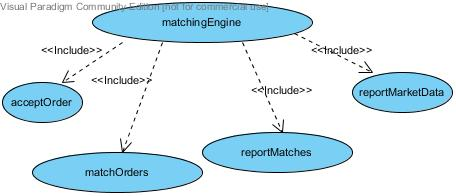
\includegraphics[scale=0.8]{./matching_engine_use_case}
						\caption{Use case for the matching engine}
						\label{matching engine use case}
						\end{figure}
				\pagebreak
				\subsubsection{Allow for multiple market participants}
				\begin{itemize}
					\item Requirement Prioritization: Critical
					\item Requirement Source: Client
					\item Requirement Level: High 	
				\end{itemize}
				Enable multiple market participants to be active in the market and allow for concurrent bids and offers to be placed. With this functionality, we can see how the market performs under certain(e.g. conditions when a stock is trending or when the market is liquid). 
				
				\subsubsection{Algorithmic trading entities}
				\begin{itemize}
					\item Requirement Prioritization: Critical
					\item Requirement Source: Client 	
					\item Requirement Level: High
				\end{itemize}
				Since there are multiple participants who will be competing in the market, we need to see how trading stategies perform in different market conditions. Each entity will need to do the following:
					\begin{itemize}
						\item Process market data and trading events from the matching engine
						\item Decide the entry or exit point into the market using data from the matching engine.
					\end{itemize}
			\pagebreak	
				\subsubsection{User Interfaces}
				\begin{itemize}
					\item Requirement Prioritization: Critical
					\item Requirement Source: Client 
					\item Requirement Level: High	
				\end{itemize}
				This requirement should provide the following user interfaces:
					\begin{itemize}
						\item  For displaying the various metrics of the performance of any selected market participant for comparing the different algorithms' performance.
						\item For showing the full market depth and matching orders by the matching engine.
					\end{itemize}

		\subsection{Domain Objects}		  
			\begin{figure}[th]
			\centering
			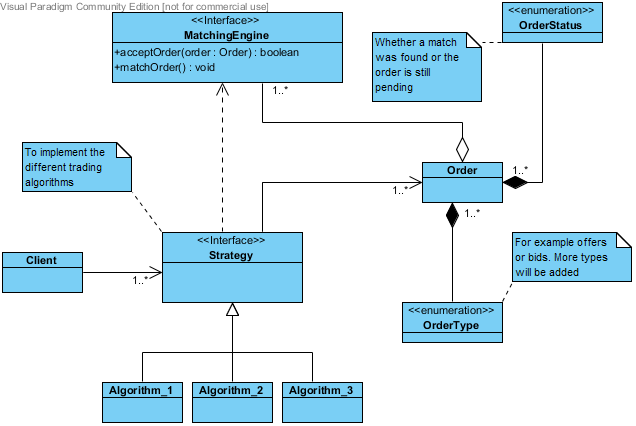
\includegraphics[scale=0.8]{./domain_objects}
			\caption{Core domain objects}
			\label{domain objects}
			\end{figure}
								
			The strategy design pattern will be used for implementing the different trading algorithms to provide pluggability.
	\newpage				
	\section{Glossary}	
		\begin{itemize}
			\item \textbf{Order}: An instruction from a participant to either put in an offer or a bid.
			\item \textbf{Market data}: Data reflecting current trading information to include pricing and volume and other additional information related to the trade.
			\item \textbf{Match}: When an offer and a bid have the same price.
		\end{itemize}				    			    			    		
\end{document}